\documentclass{beamer}

\usepackage{soul}
\usepackage{minted}
\usepackage[font=small,labelfont=bf]{caption}
\usepackage{graphics}
\graphicspath{{./images/}}
\usetheme{metropolis}

\title{Why should you use Rust}
\date{\today}
\author{Vlad Aleksashyn}
\institute{Apriorit Dev Club 33}

\begin{document}

\maketitle

\section{Intro}
    \begin{frame}{About me}
        \begin{itemize}
            \item Vlad Aleksashyn
            \item Software Designed at Apriorit
            \item Mostly work with virtualization, Linux kernel and native
            \item Used to love C++ a lot, still love C
            \item Started using Rust at 2016 and regreat nothing
            \item Developed a real-time GPU ray tracer with Rust and Vulkan
            \item Now developing image compression library for RPD in Rust
        \end{itemize}
        Contact:
        \begin{itemize}
            \item GitHub: vaffeine
            \item Email: vlad.al.dp@gmail.com
            \item Skype: vlad.aleks
        \end{itemize}
    \end{frame}

    \begin{frame}{About Rust}
        \begin{columns}
        \column{0.7\textwidth}
            \begin{itemize}
                \item Started by Graydon Hoare in 2006
                \item Named after the rust family of fungi (?)
                \item First appeared July 7, 2010
                \item Successfully compiled itself in 2011
                \item First stable release 1.0 / May 15, 2015
                \item Was the 3rd most loved programming language in the 2015 Stack Overflow annual survey
                \item \ldots and took first place in 2016, 2017, and 2018.
                \item Stable release 1.30.1 / November 8, 2018
            \end{itemize}
        \column{0.3\textwidth}
            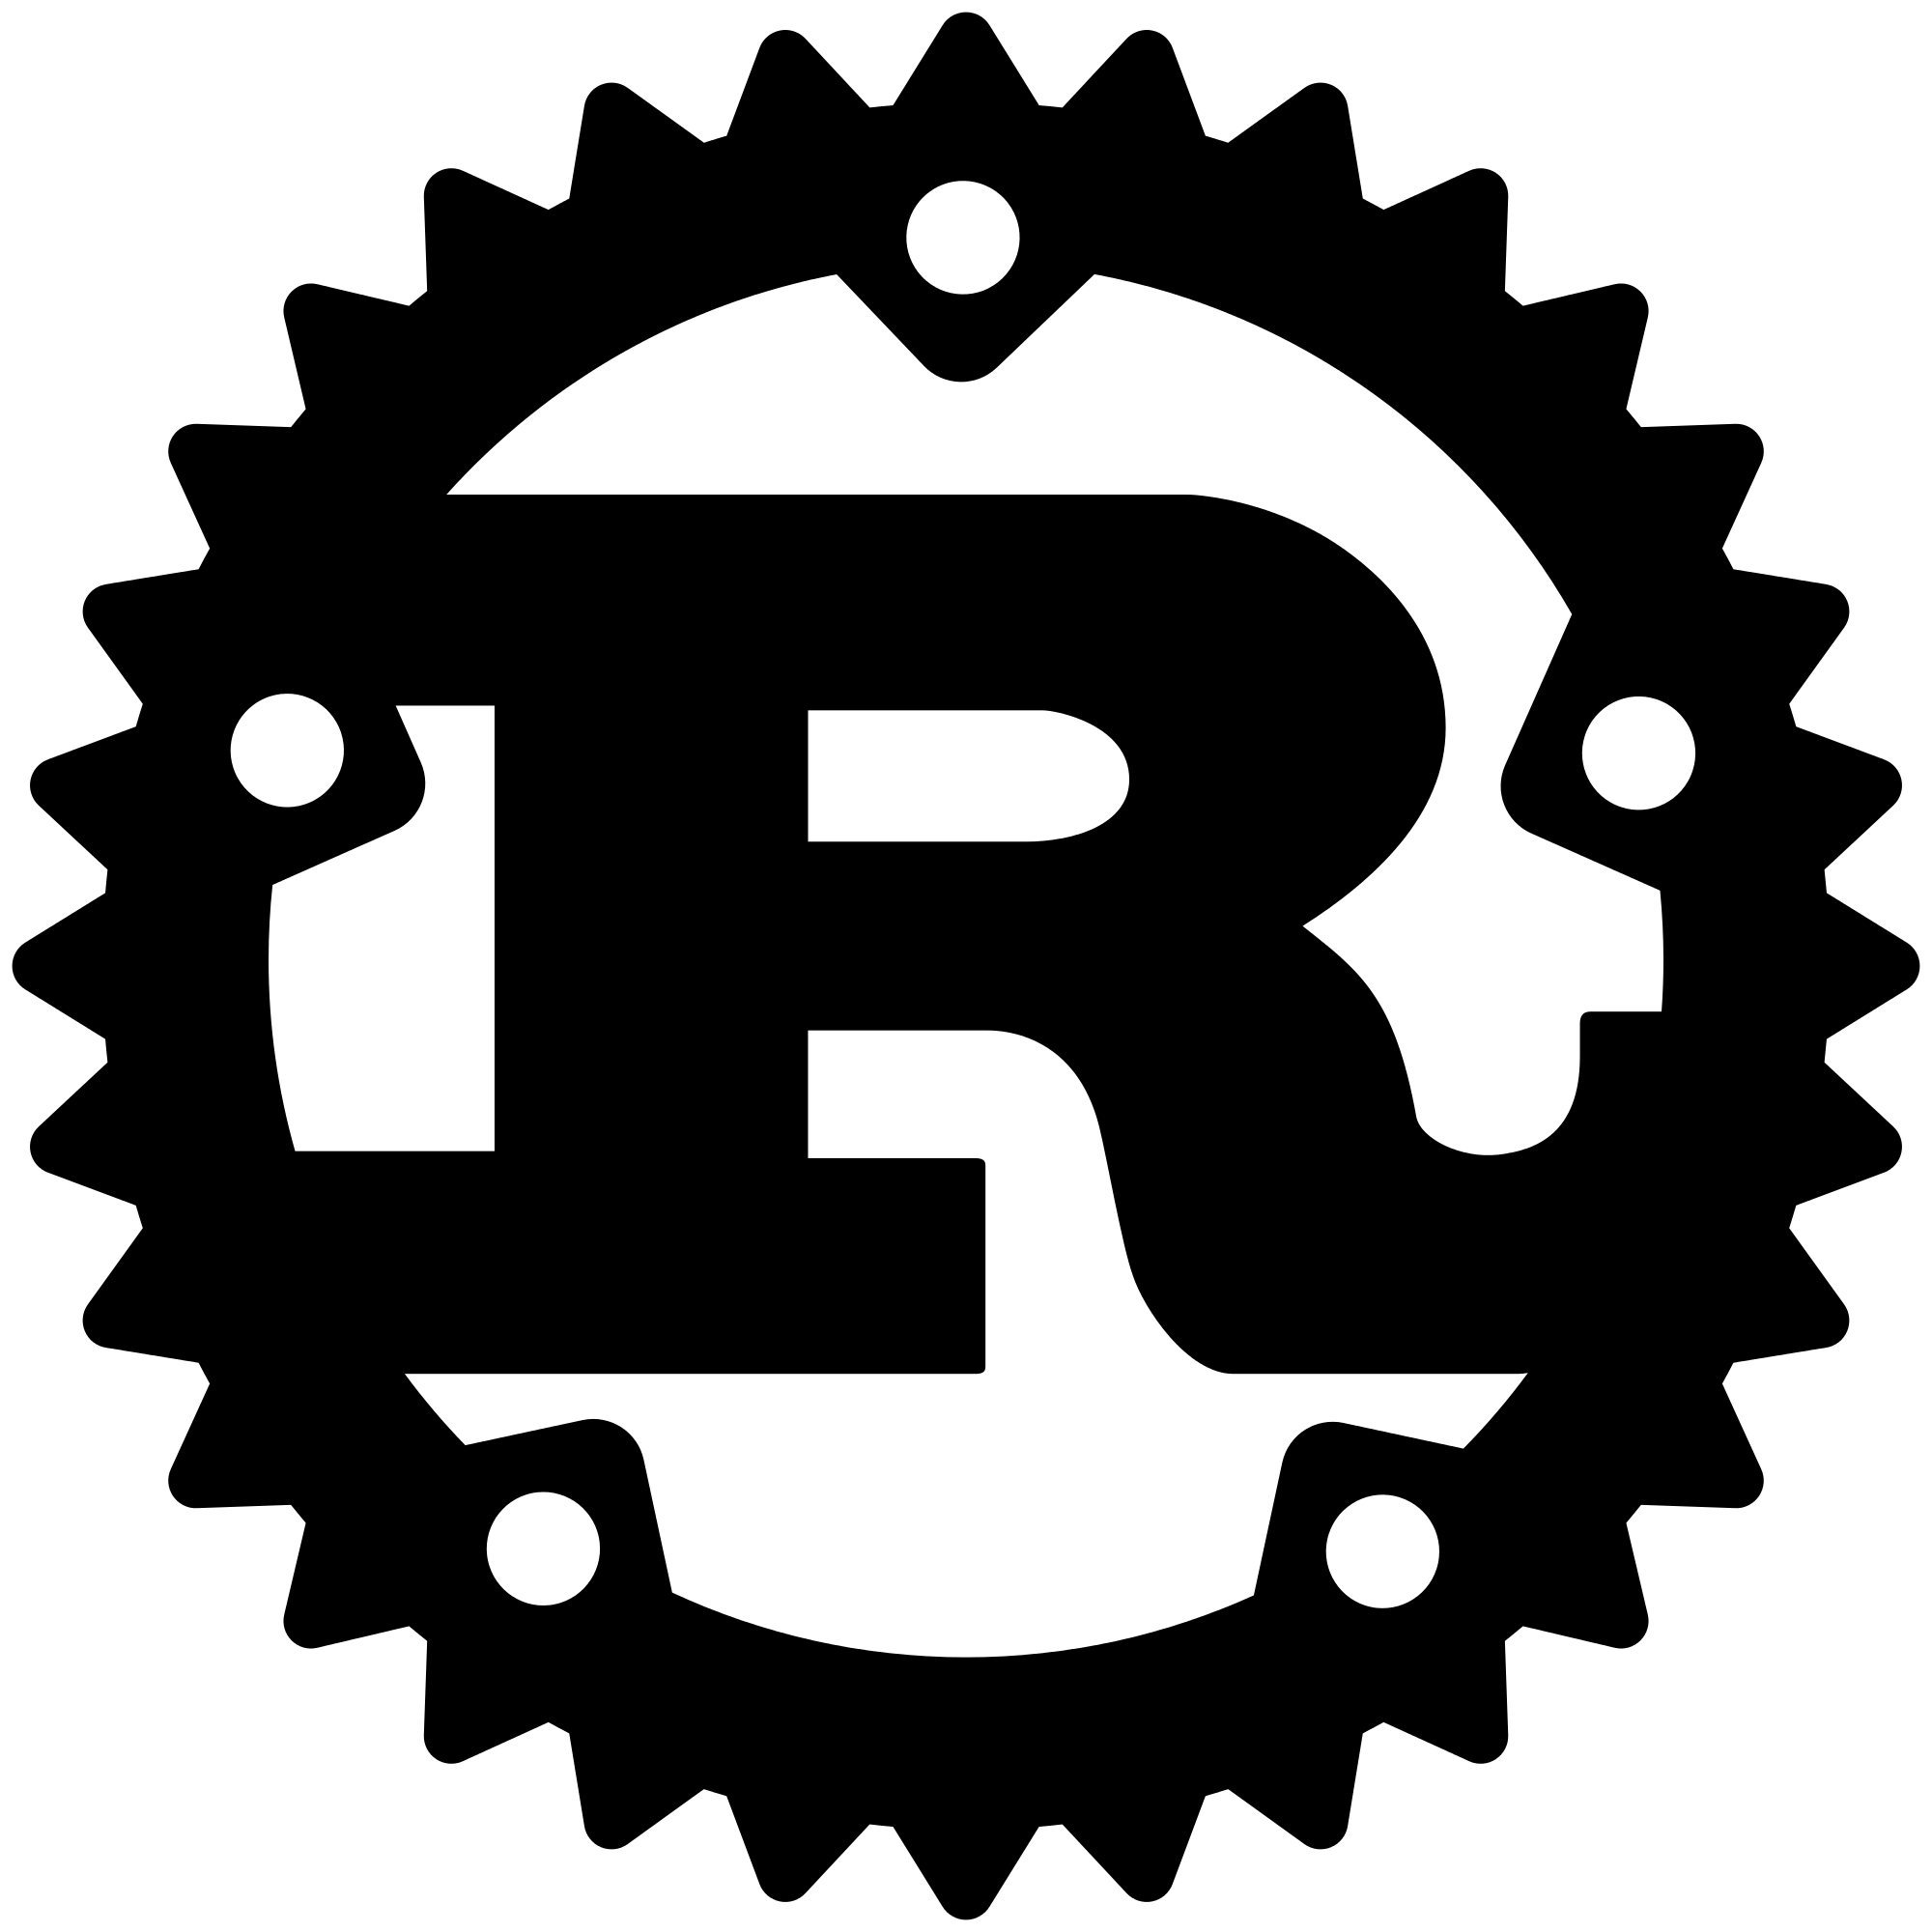
\includegraphics[width=\textwidth]{rust_logo}
            \captionof{figure}{Rust logo}
        \end{columns}
    \end{frame}

    \begin{frame}[fragile]{Code example \#1}

        \large\begin{minted}{rust}
extern crate rand; // external library

use rand::Rng;

fn main() {
    let mut rng = rand::thread_rng();

    let numbers: Vec<i64> = (0..100)
        .map(|_| rng.gen_range(1, 42))
        .collect();

    println!("{:?}", numbers);
}
        \end{minted}

    \end{frame}

    \begin{frame}[fragile]{Code example \#2}
        \vfill
        \large\begin{minted}{rust}
enum Event {
    Load,
    KeyPress(char),
    Click { x: i64, y: i64 }
}

fn process_event(event: Event) {
    match event {
        Event::Load => ...,
        Event::KeyPress(c) => ...,
        Event::Click {x, y} => ...,
    }
}
        \end{minted}

    \end{frame}

    \begin{frame}{Companies that use Rust}
        \vfill
        \begin{columns}
        \column{0.3\textwidth}
            \vbox to 0.5\textheight{
                
\includegraphics[width=\textwidth]{dropbox}
                \vfill
                
\includegraphics[width=\textwidth]{smartthings}
                \vfill
                
\includegraphics[width=\textwidth]{atlassian}
            }
        \column{0.3\textwidth}
            \vbox to 0.6\textheight{
                
\includegraphics[width=\textwidth]{habitat}
                \vfill
                
\includegraphics[width=\textwidth]{mozilla}
                \vfill
                
\includegraphics[width=\textwidth]{npm}
            }
        \column{0.3\textwidth}
            \vbox to 0.7\textheight{
                
\includegraphics[width=\textwidth]{threatx}
                \vfill
                
\includegraphics[width=\textwidth]{devolutions}
                \vfill
                
\includegraphics[width=\textwidth]{apriorit}
            }
        \end{columns}
        And many many more\dots

        Visit https://www.rust-lang.org/en-US/friends.html
    \end{frame}

\section{TRust}

    \begin{frame}{Linux CVEs in 2018}
        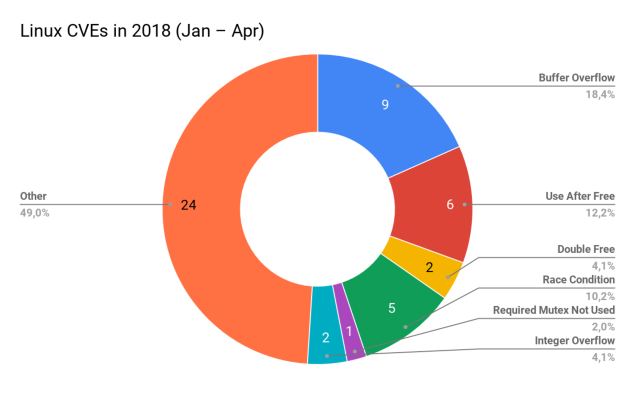
\includegraphics[width=\textwidth]{linux_cves_2018}
        \captionof{figure}{https://phil-opp.github.io/talk-konstanz-may-2018}
    \end{frame}

    \begin{frame}{Memory Safety}
        \Large{
            \begin{itemize}
                \item No buffer overflows*
                \item No dangling pointers
                \item No data races
            \end{itemize}
            \vfill
            Guaranteed by Rust's ownership system
            \underline{at compile time!}
        }
        \vfill
        \vfill
        \small{* unless you explicitly want them}
    \end{frame}

    \begin{frame}[fragile]{Fearless concurency}
        \vfill
        \begin{columns}
        \column{0.5\textwidth}
            C++
            \vfill
            \noindent\rule{\textwidth}{1pt}
            \small\begin{minted}{cpp}
std::vector data = {1, 2, 3};
// mutex is unrelated to data
std::mutex mutex;
...
// unsynchronized access
data.push_back(4);

// can forget to use lock guard
std::lock_guard lock(mutex);
data.push_back(5);
            \end{minted}
            \noindent\rule{\textwidth}{1pt}
        \column{0.5\textwidth}
            Rust
            \vfill
            \noindent\rule{\textwidth}{1pt}
            \small\begin{minted}{rust}
let data = vec![1, 2, 3];
// data is moved inside mutex
let mutex = Mutex::new(data);

// compilation error
data.push(4);

// can't access data w/o lock
let mut d = mutex.lock()?;
d.push(5);
            \end{minted}
            \noindent\rule{\textwidth}{1pt}
        \end{columns}
        Rust ensures that Mutex is locked before accessing data
    \end{frame}

    \begin{frame}{Encapsulating Unsafety}
        Not everything can be verified at compile time.

        For this cases Rust has unsafe blocks that allow to
        \begin{itemize}
            \item Dereference raw pointers
            \item Call unsafe functions
            \item Access mutable statics
            \item Implement unsafe traits
        \end{itemize}
        but only in this block.
    \end{frame}

\section{Convenience}

    \begin{frame}[fragile]{Clean generics}
        \vfill
        \begin{columns}
        \column{0.5\textwidth}
            C++
            \vfill
            \noindent\rule{\textwidth}{1pt}
            \large{
                \begin{minted}{cpp}
class MyType {};
unordered_set<MyType>;
                \end{minted}
            }
            \noindent\rule{\textwidth}{1pt}
            \vfill
            191 lines of compile errors with only 2 of them being usefull.

            But there will be contracts in \st{C++17} \st{C++20} C++24.
        \column{0.5\textwidth}
            Rust
            \vfill
            \noindent\rule{\textwidth}{1pt}
            \large{
                \begin{minted}{rust}
struct MyType;
HashSet::<MyType>::new();
                \end{minted}
            }
            \noindent\rule{\textwidth}{1pt}
            \vfill
            the following trait bounds were not satisfied:

            \small{
                `foo::MyType : std::cmp::Eq`

                `foo::MyType : std::hash::Hash`
            }
        \end{columns}
    \end{frame}

    \begin{frame}[fragile]{Cool iterators and closures}

        Take the values produced by an instance of Counter,
        pair them with values produced by another Counter instance
        after skipping the first value, multiply each pair together,
        keep only those results that are divisible by 3,
        and add all the resulting values together:

        \large\begin{minted}{rust}
let sum: u32 = Counter::new()
     .zip(Counter::new().skip(1))
     .map(|(a, b)| a * b)
     .filter(|x| x % 3 == 0)
     .sum();

assert_eq!(18, sum);
        \end{minted}

    \end{frame}

    \begin{frame}[fragile]{Effective error handling}

        \large\begin{minted}{rust}
use std::io::{self, Read};
use std::fs::File;

fn read_username_from_file()
                -> io::Result<String> {
    let mut s = String::new();

    File::open("hello.txt")?
        .read_to_string(&mut s)?;

    Ok(s)
}
        \end{minted}
    No exceptions are needed!

    \end{frame}

    \begin{frame}[fragile]{Modules system}
        Project structure:

        \large{
            \begin{itemize}
                \item src
                \begin{itemize}
                    \item client.rs
                    \item lib.rs
                    \item network
                    \begin{itemize}
                        \item mod.rs
                        \item server.rs
                    \end{itemize}
                \end{itemize}
            \end{itemize}
        }
        \large\begin{minted}{rust}
// lib.rs
mod client;
mod network;

pub use network::Server;
pub use client::Client;
        \end{minted}
    \end{frame}

\section{Tools}

    \begin{frame}{Cargo}
        \begin{columns}
        \column{0.6\textwidth}
            \large{
                \begin{itemize}
                    \item Over 15000 crates on crates.io
                    \item Simply specify the desired version
                    \begin{itemize}
                        \item Add single line to Cargo.toml
                    \end{itemize}
                    \item Cargo takes care of the rest
                    \begin{itemize}
                        \item Downloading, building, linking
                    \end{itemize}
                \end{itemize}
            }
        \column{0.4\textwidth}
            
\includegraphics[width=\textwidth]{cargo-logo}
            \captionof{figure}{Cargo logo}
        \end{columns}
    \end{frame}

    \begin{frame}{Tools}
        \begin{itemize}
            \item rustup: Use multiple Rust versions for different directories
            \item rustfmt: Format Rust code according to style guidelines
            \item clippy: Additional warnings for dangerous or unidiomatic code
            \item Rust Playground: Run and share code snippets in your browser
        \end{itemize}
		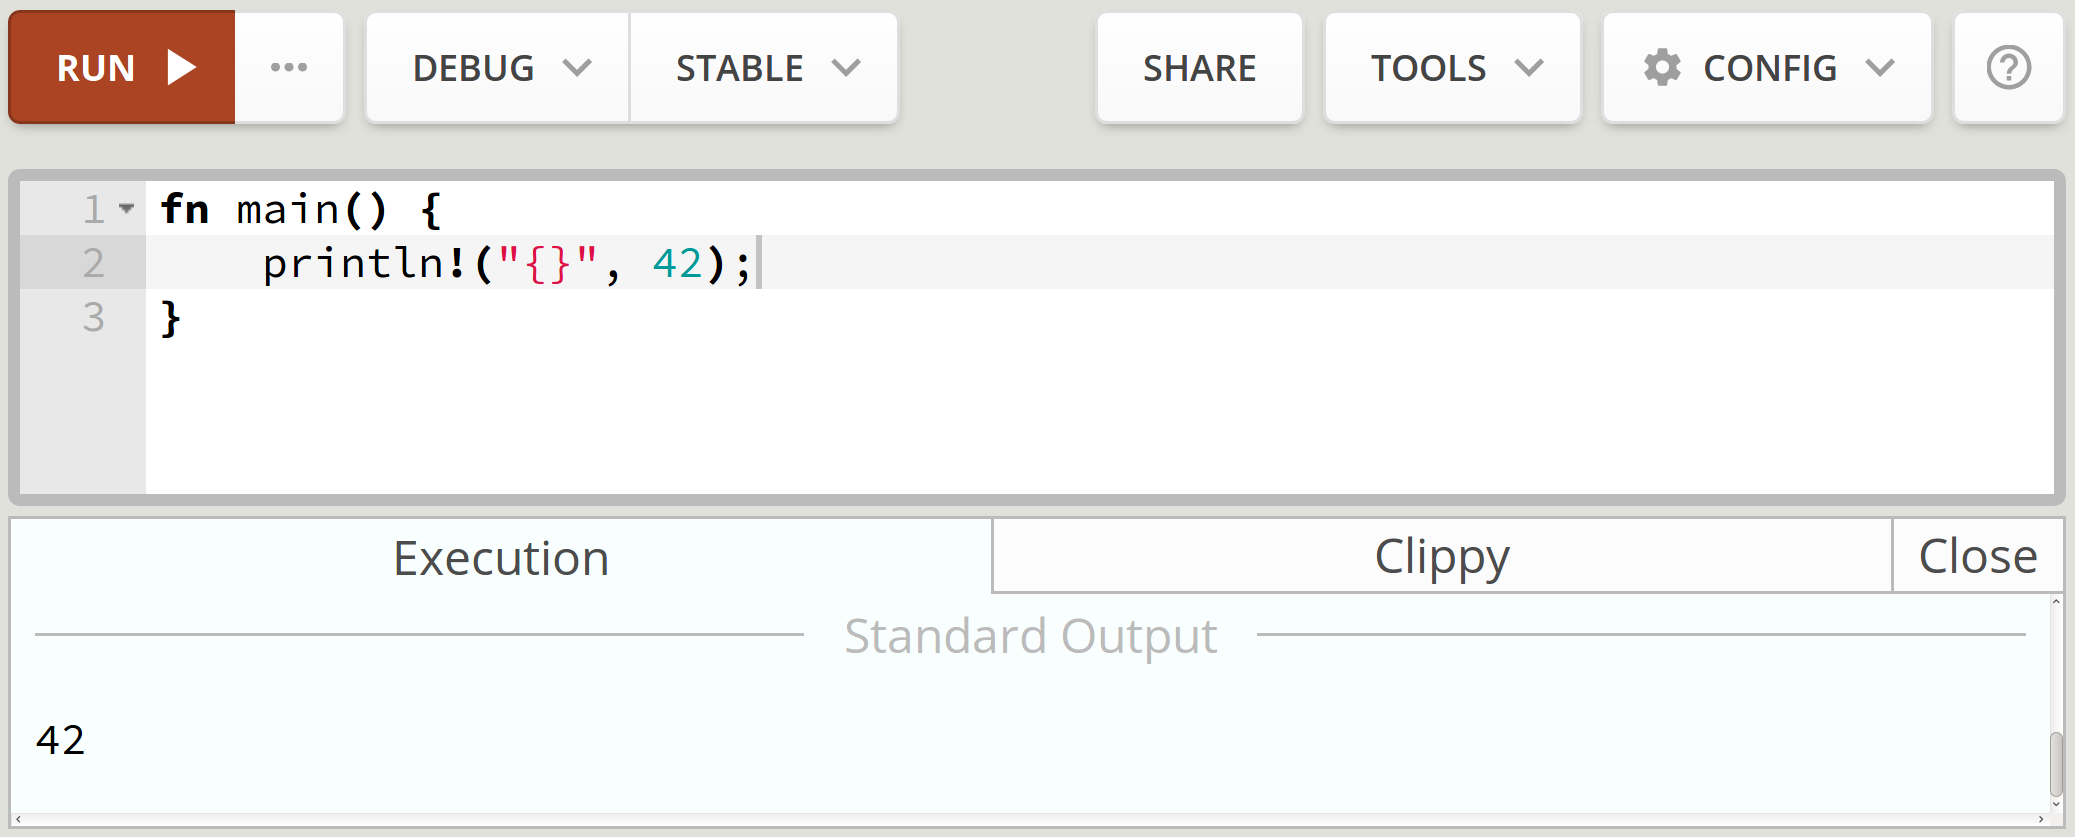
\includegraphics[width=\textwidth]{playground}
    \end{frame}

    \begin{frame}[fragile]{Testing}
		Built-in testing framework:
        \large\begin{minted}{rust}
fn add_two(a: i32) -> i32 {
	a + 2
}

#[test]
fn test_add_two() {
	assert_eq!(4, add_two(2));
}

#[bench]
fn bench_add_two(b: &mut Bencher) {
	b.iter(|| add_two(2));
}
        \end{minted}
    \end{frame}

\section{What can I use Rust for?}
    \begin{frame}{Native applications}
		Tier 1:
		\begin{itemize}
			\item x86 Linux 2.6.18+
			\item x86 OSX 10.7+
			\item x86 Windows 7+
		\end{itemize}

		Tier 2:
		\begin{itemize}
			\item ARM64
			\item ARMv5-ARM7
			\item MIPS and MIPS64
			\item PowerPC
			\item on Linux, FreeBSD, NetBSD, Android and iOS
		\end{itemize}
    \end{frame}

	\begin{frame}{Kernel, bootloader, firmware, etc.}
		\begin{itemize}
			\item You can compile Rust without standard library
			\item You will still have plenty of features from Core library
			\item Take a look at tutorials by Philipp Oppermann and Redox OS
		\end{itemize}
		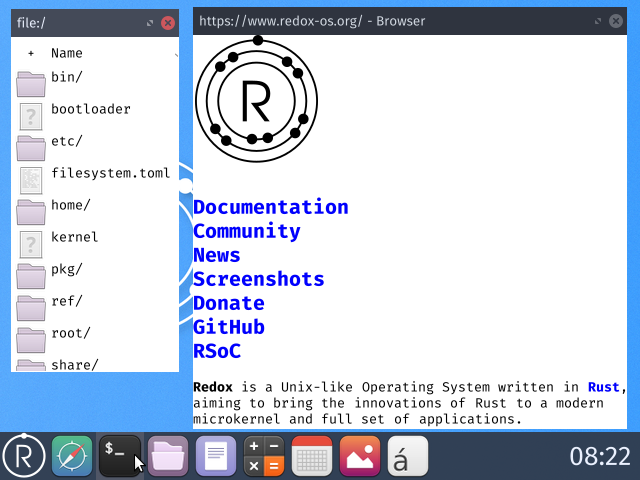
\includegraphics[height=0.5\textheight]{redox}
    \end{frame}

	\begin{frame}[fragile]{Networking}
		Cool low level async networking with tokio.rs:
        \small\begin{minted}{rust}
let listener = TcpListener::bind(&addr)?;

let server = listener.incoming()
	.map_err(|e| eprintln!("error"))
	.for_each(|sock| {
		let (reader, writer) = sock.split();
		let bytes_copied = copy(reader, writer);
		let handle_conn = bytes_copied.map(|amt| {
			println!("wrote {:?} bytes", amt)
		}).map_err(|err| {
			eprintln!("IO error {:?}", err)
		});
		tokio::spawn(handle_conn)
	});
tokio::run(server);
        \end{minted}
    \end{frame}

	\begin{frame}[fragile]{Web applications}
		Safety aimed web framework Rocket:
        \large\begin{minted}{rust}
#[get("/<name>/<age>")]
fn hello(name: String, age: u8) -> String {
	format!("Hello, {} year old named {}!",
			age, name)
}

fn main() {
	rocket::ignite()
		.mount("/hello", routes![hello])
		.launch();
}
        \end{minted}
    \end{frame}

	\begin{frame}[fragile]{Web client code}
		There are only 3 languages, that could be compiled to WebAssembly
		and run in client's web browser:
		\begin{itemize}
			\item C
			\item C++
			\item Rust
		\end{itemize}
    \end{frame}

\section{QA}

\end{document}
